\documentclass[aspectratio=169]{beamer}

\usepackage[utf8]{inputenc}
\usepackage{amsmath}
\usepackage{amsfonts}
\usepackage{amssymb}
\usepackage{graphicx}
\usepackage{ragged2e}  % `\justifying` text
\usepackage{booktabs}  % Tables
\usepackage{tabularx}
\usepackage{tikz}      % Diagrams
\usetikzlibrary{calc, shapes, backgrounds}
\usepackage{amsmath}
\usepackage{amssymb}
\usepackage{dsfont}
\usepackage{url}       % `\url
\usepackage{listings}  % Code listings
\usepackage[T1]{fontenc}
% \usepackage{subfig}
\usepackage{subcaption}
\usepackage{theme/beamerthemehbrs}

\author[Lau]{Wing Ki Lau}
\title{R\&D project defense}
\subtitle{Exploiting contact constraints in robotic manipulation tasks}
\institute[HBRS]{Hochschule Bonn-Rhein-Sieg}
\date{\today}
\subject{Test beamer}

% leave the value of this argument empty if the advisors
% should not be included on the title slide
\def\advisors{Prof. Dr. Nico Hochgeschwender, M.Sc. Sven Schneider}

% \thirdpartylogo{path/to/your/image}
% \usepackage[backend=bibtex,citestyle=verbose-ibid,style=authoryear-ibid]{biblatex}%Imports biblatex 
\usepackage[backend=bibtex,style=ieee]{biblatex}
\addbibresource{bibliography.bib}

\begin{document}
{
\begin{frame}
\titlepage
\end{frame}
}


\section{First section}
\subsection{A subsection}

\begin{frame}{Introduction}
    \framesubtitle{Human vs robot}
    \begin{figure}
      \subfloat[Picture of human writing \cite{Says_2022}]{
      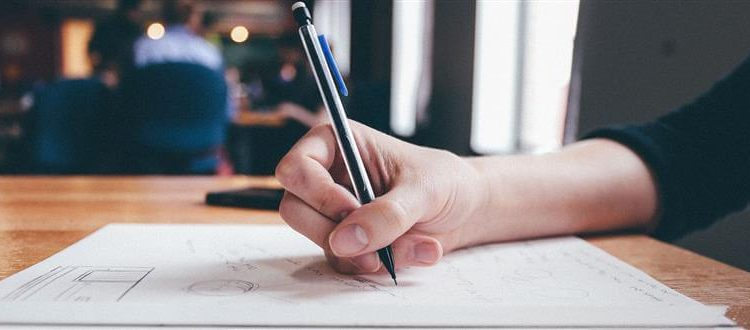
\includegraphics[width=0.45\textwidth]{images/human_write.jpg}}
      \hspace{0.5em}
      \subfloat[The example of robot performing writing \cite{Newton_2017}]{
      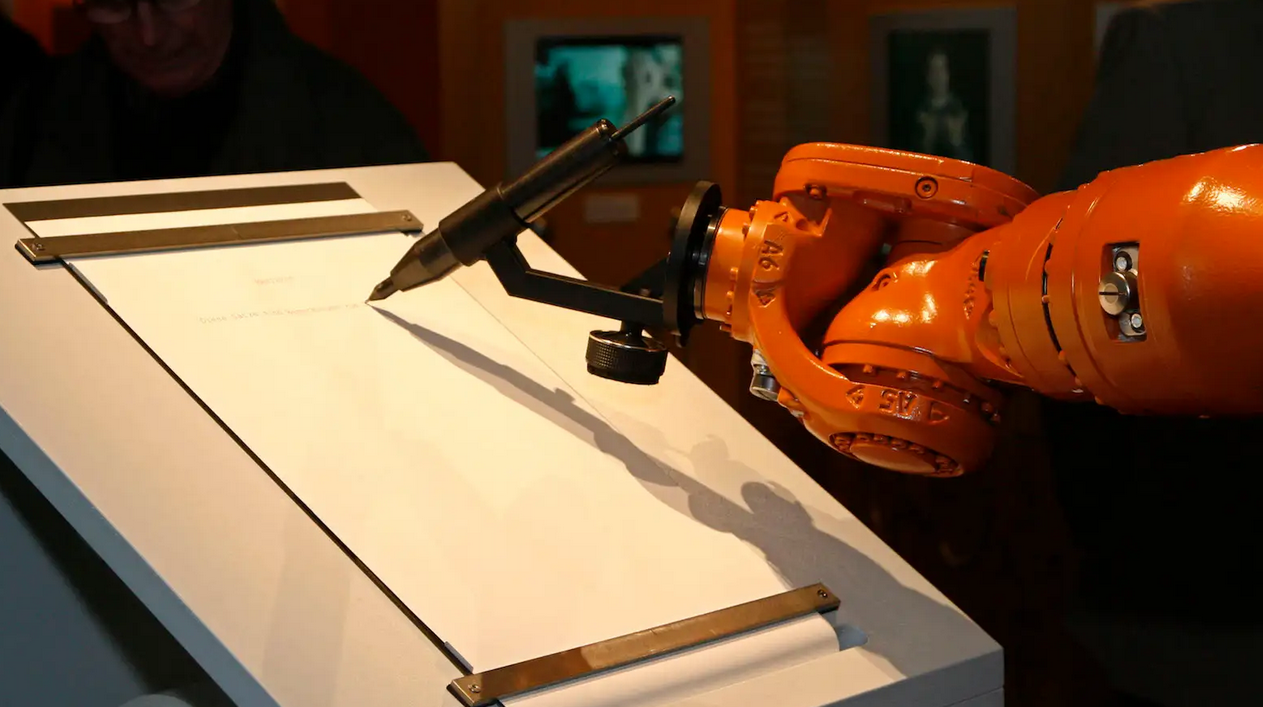
\includegraphics[width=0.45\textwidth]{images/robot_write.png}}
    \end{figure}
\end{frame}


\begin{frame}{Current work}
  \begin{itemize}
    \item Articulated Body Algorithm (ABA)
    \begin{itemize}
      \item Solve forward dynamics problem hierarchically \cite{featherstone1983calculation}
      \item Does not support partial task specifications for bias force 
    \end{itemize}
    \item Recursive Newton-Euler algorithm (RNEA)
    \begin{itemize}
      \item Solve inverse dynamics problem recursively \cite{featherstone2007book} \cite{featherstone1999divide}
      \item Require task specification in all 6 directions when defining constraints
    \end{itemize}
\end{itemize}
\end{frame}

\begin{frame}{Current work}
    \framesubtitle{Popov-Vereshchagin hybrid-dynamics (PV) solver }
  \begin{itemize}
    \item Exploite the defined constraints,robot model, joint angles, joint velocities, feed forward torque and external forces to compute the required joint torque and joint accelerations \cite{vereshchagin1989modeling} 
    \item Allow to use task definitions directly as input \cite{vereshchagin1974computer}:
    \begin{enumerate}
      \item Cartesian Acceleration constraints : $\alpha_N^T \ddot{X_N} = \beta_N$
      \item The virtual and physical external force acting on each segments: $F_{ext}$
      \item The feed-forward force $\tau$ acts on each joint
    \end{enumerate}
    \item Not widely noticable in academia 
    \item Lack concreate application \cite{kulkarni2019applying}
\end{itemize}
\end{frame}

\begin{frame}{Current work}
  \framesubtitle{PV solver - Cartesian Acceleration constraints}
  % \begin{center}
  %   \vspace{-20mm}
  %   $\alpha_N^T \ddot{X_N} = \beta_N$
  % \end{center}
  \vspace{-15mm}
  \begin{block}{The structure of Cartesian Acceleration constraints}
    
    $\alpha_N^T \ddot{X_N} = \beta_N$
  \end{block}
\begin{itemize}
  \item Manage physical interactions with the environment
  \item Deal with artificial constraints
\end{itemize}
\vspace{-3mm}
\begin{figure}
  \subfloat[Number of constraint = 1]{
  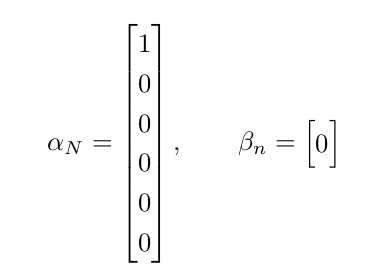
\includegraphics[width=0.3\textwidth]{images/ab1.png}}
  \hspace{2mm}
  \subfloat[A full contraint]{
  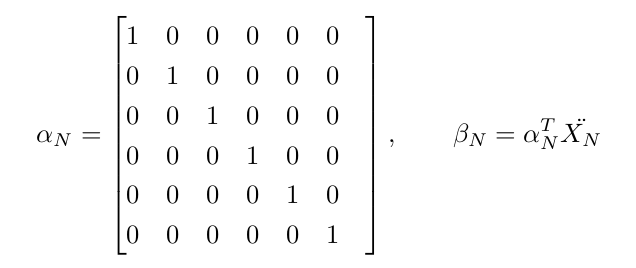
\includegraphics[width=0.5\textwidth]{images/abfull.png}}
\end{figure}
\vspace{-30mm}
\end{frame}

\begin{frame}{Robot architecture}
\centering
\begin{figure}
  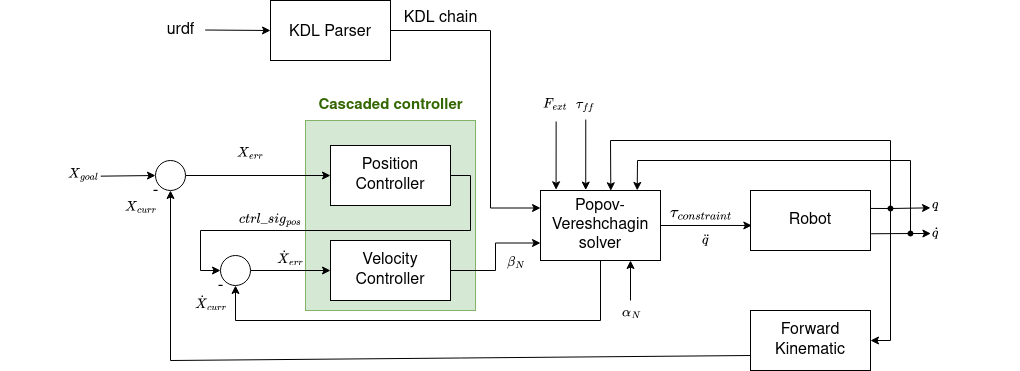
\includegraphics[width=0.95\textwidth]{images/system_arch.png}
  \caption{A generic robot system architecture}
\end{figure}
% \vspace{-15mm}
\end{frame}


\defverbatim[colored]\sleepSort{
\begin{lstlisting}[language=C,tabsize=1,basicstyle=\scriptsize,xleftmargin=.3\textwidth]
  
  struct robif2b_kinova_gen3_nbx
  {
    double *act_cur_msr; //[A]
    double *act_vol_msr; //[V]
    double *gripper_pos_msr;
    const double *gripper_pos_cmd;
  }
\end{lstlisting}
\captionof{lstlisting}{Code snipnet of new command}
}

\begin{frame}{Extension of Robif2b}
\begin{itemize}
  \item A robot control interface wraps the
  session creation, connection establishment and communication between actuator, base and client side \cite{Rosym-Project}
  \item Uncapable to retrieve the voltage and current status of the gripper actuator
  \sleepSort
\end{itemize}
\end{frame}

\begin{frame}{Experiement and evaluation}
  \begin{columns}[c]
    \begin{column}{.5\textwidth}
      Three experiements was performed:
      \begin{enumerate}
        \item Grasp object by sliding motion along surface
        \item Perform writing task
        \item Resting elbow manipulation
      \end{enumerate}     
    \end{column}
    \begin{column}{.5\textwidth}
    \begin{figure}
      \centering
      \begin{figure}
        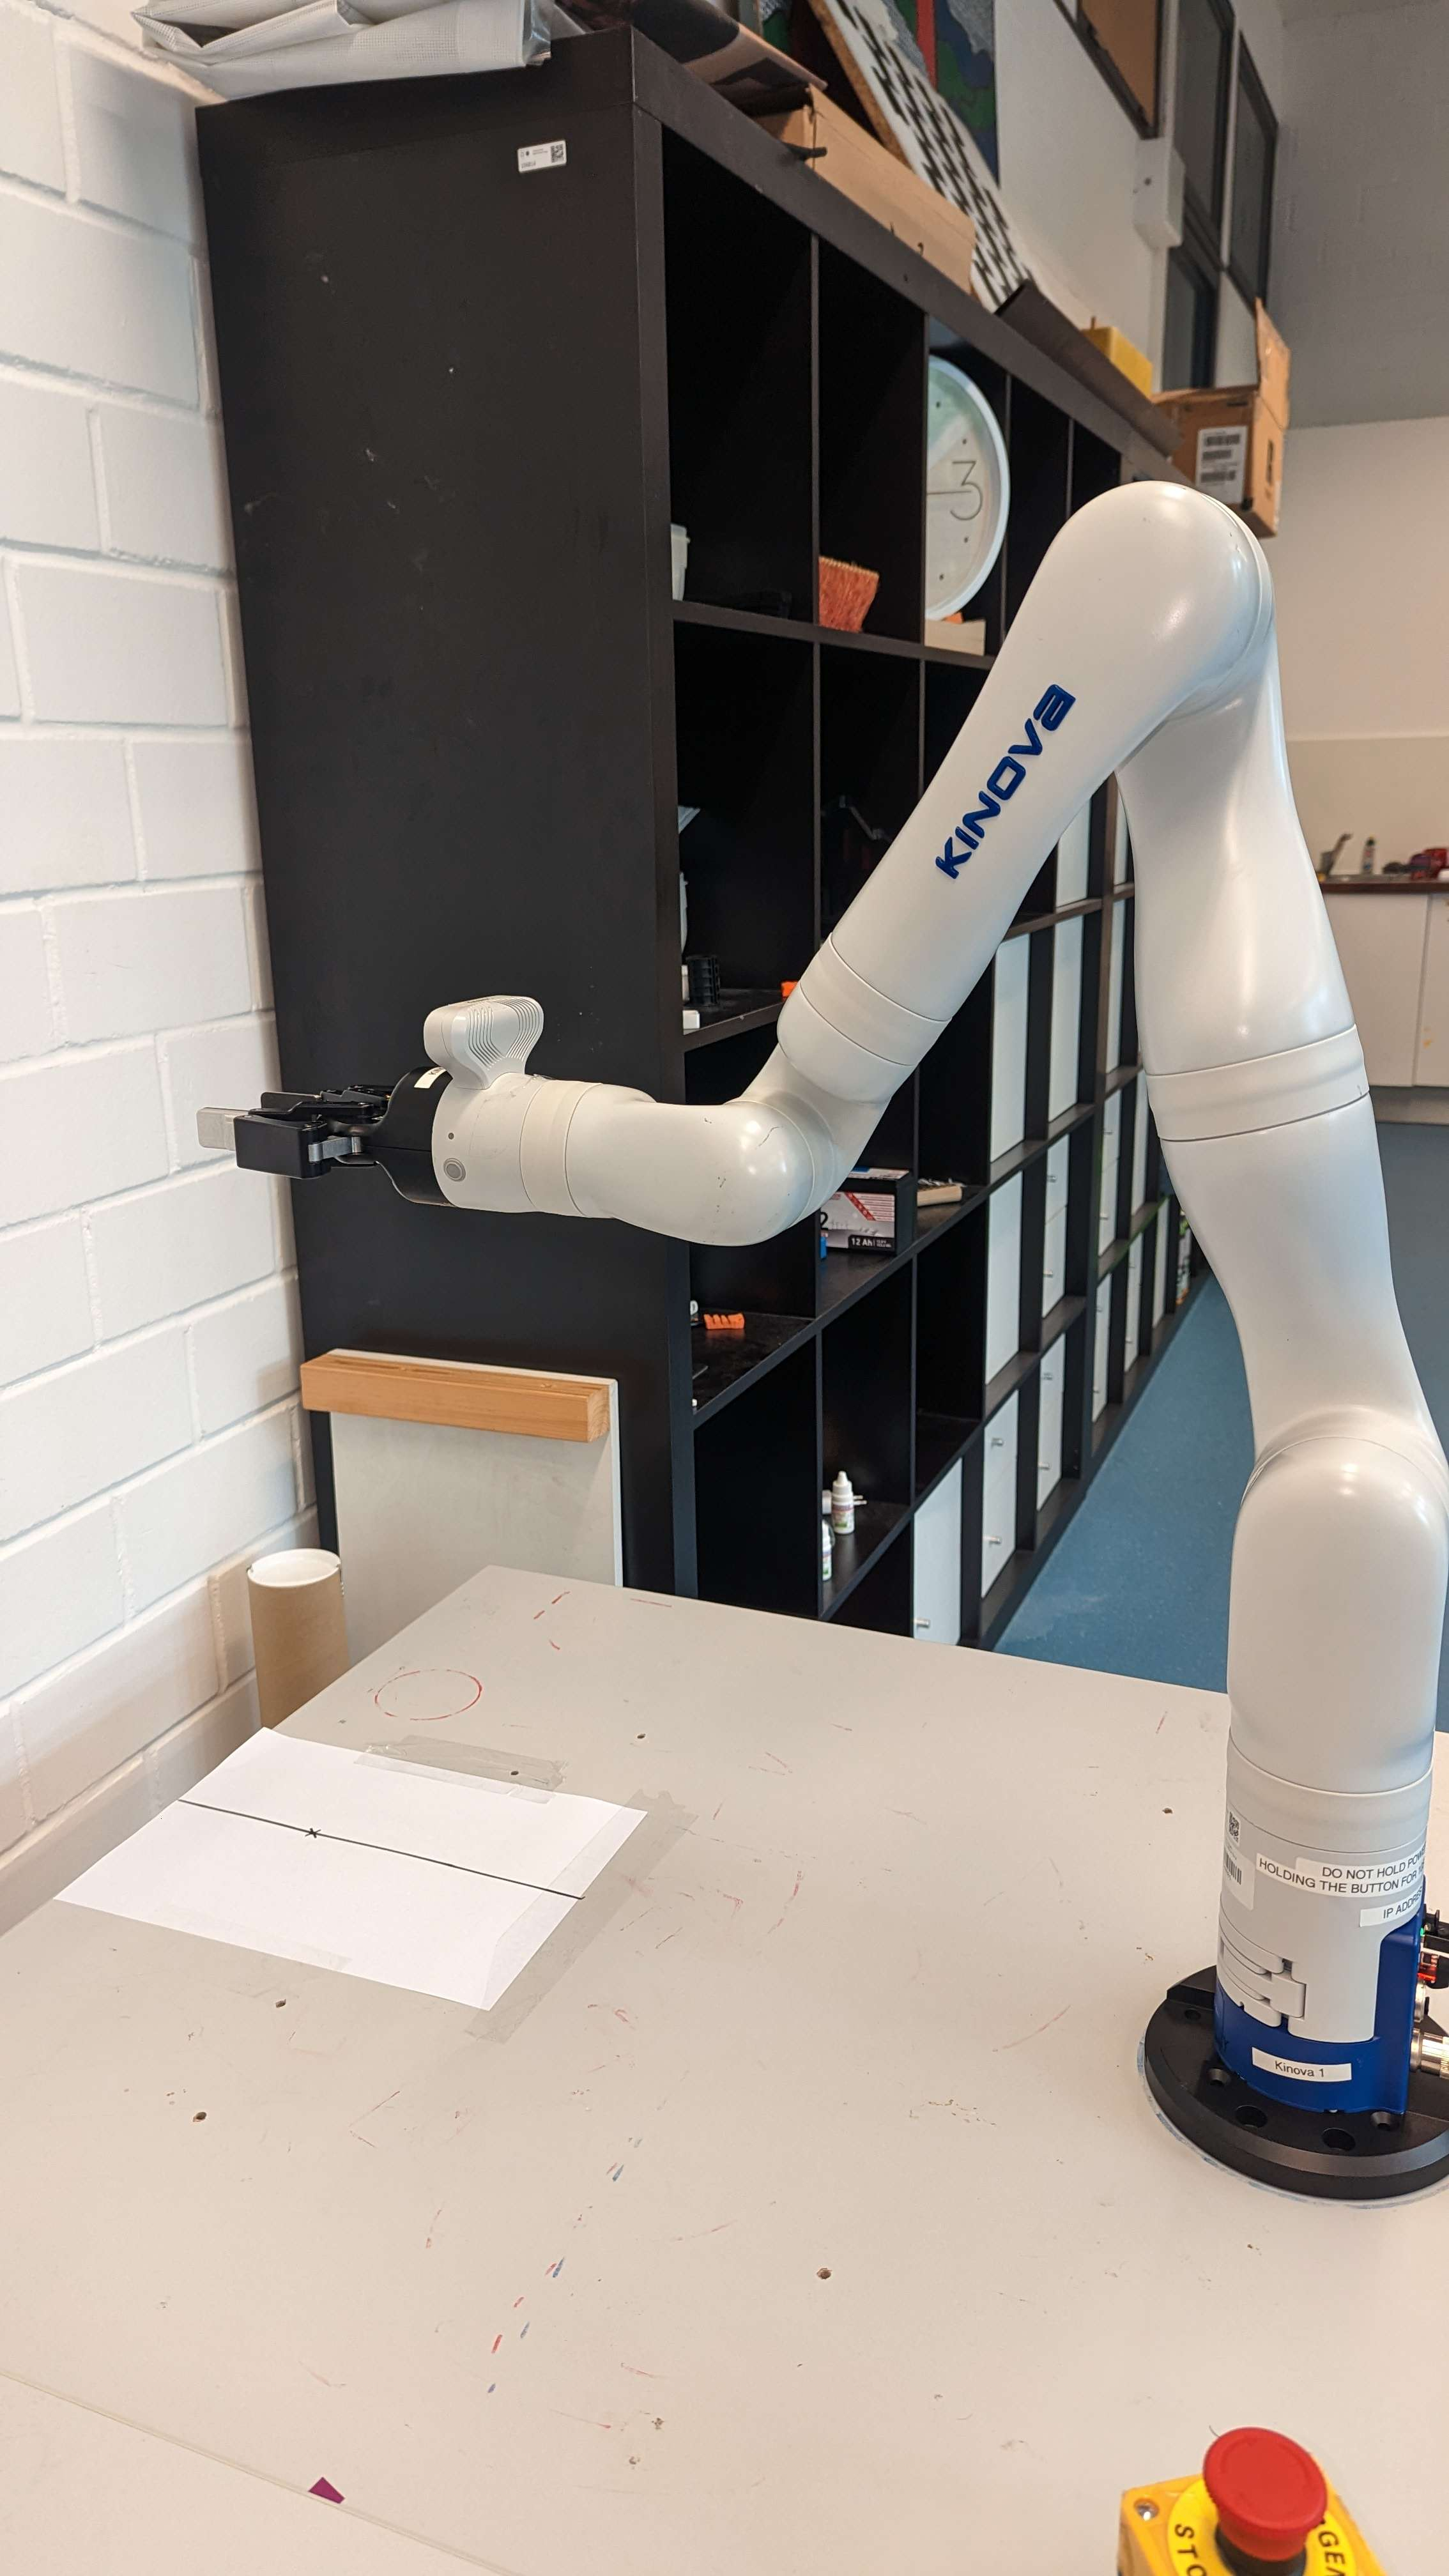
\includegraphics[width=0.5\textwidth]{images/us1_initial.jpg}
      \end{figure}
    \end{figure}
    \end{column}
    \end{columns}
  \end{frame}

  \begin{frame}{Experiement and evaluation}
    \framesubtitle{Grasp object by sliding motion along surface}
    \begin{columns}[c]
      \begin{column}{.5\textwidth}
        \begin{itemize}
          \item A proof-of-concept task
          \item Energy efficiency and joint torque will be evaluated
        \end{itemize}     
        \centering
        \begin{block}{Hypothesis}
          The energy efficiency increases and 
          joint torque decrease in contact case
        \end{block}

      \end{column}
      \begin{column}{.5\textwidth}
        \centering
        *insert demo video*
      \end{column}
      \end{columns}
  \end{frame}

  \begin{frame}{Experiement and evaluation}
    \framesubtitle{Grasp object by sliding motion along surface}
    \vspace{-5mm}
    \begin{columns}[c]
      \begin{column}{.5\textwidth}
        \begin{figure}
        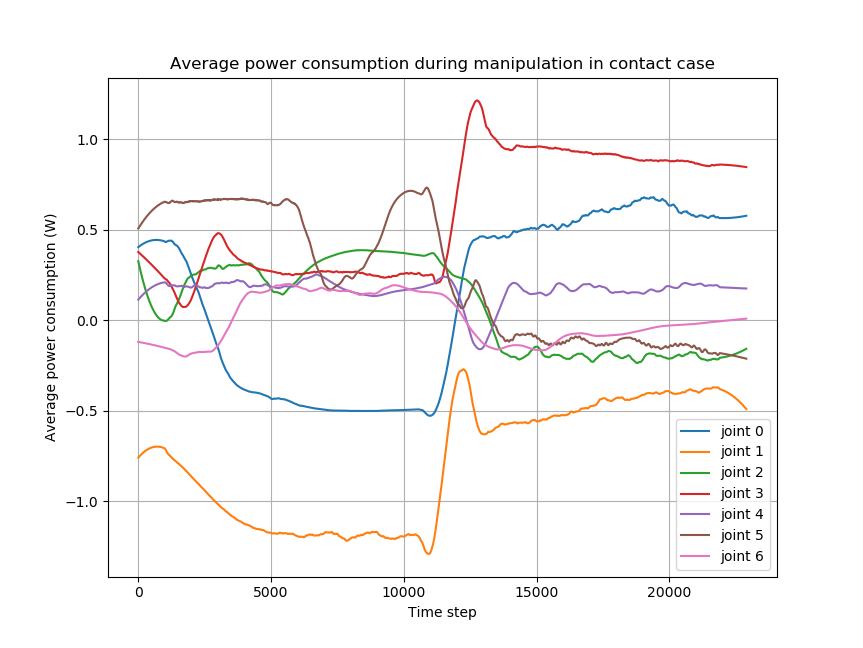
\includegraphics[width=1\textwidth]{images/us1_con_pow.png}
        \caption{Average power consumption during manipulation in contact case}
      \end{figure}
      \end{column}
      \begin{column}{.5\textwidth}
      \begin{figure}
        \centering
        \begin{figure}
          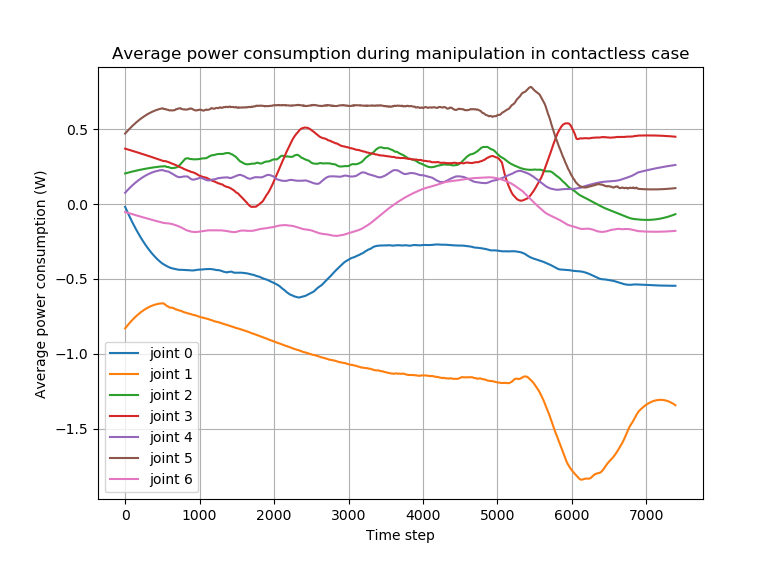
\includegraphics[width=1\textwidth]{images/us1_conless_pow.png}
          \caption{Average power consumption during manipulation in contactless case}
        \end{figure}
      \end{figure}
      \end{column}
      \end{columns}
  \end{frame}

  \begin{frame}{Experiement and evaluation}
    \framesubtitle{Grasp object by sliding motion along surface}
    \vspace{-5mm}
    \begin{columns}[c]
      \begin{column}{.5\textwidth}
        \begin{figure}
        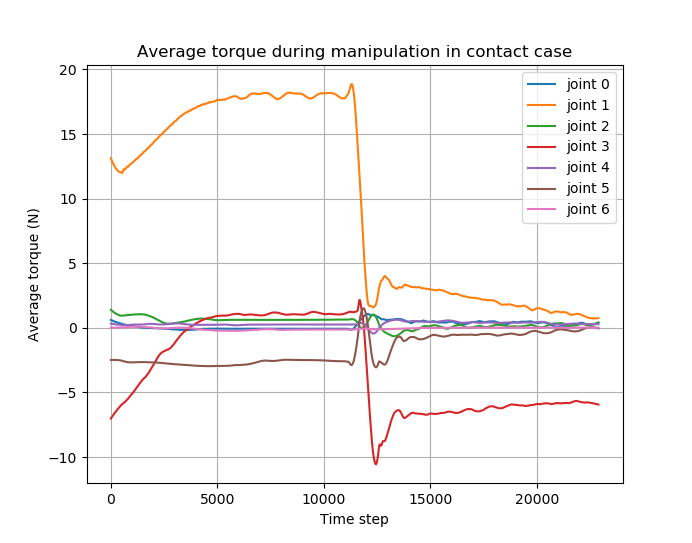
\includegraphics[width=1\textwidth]{images/us1_con_tor.png}
        \caption{Average torque during manipulation in contact case}
      \end{figure}
      \end{column}
      \begin{column}{.5\textwidth}
      \begin{figure}
        \centering
        \begin{figure}
          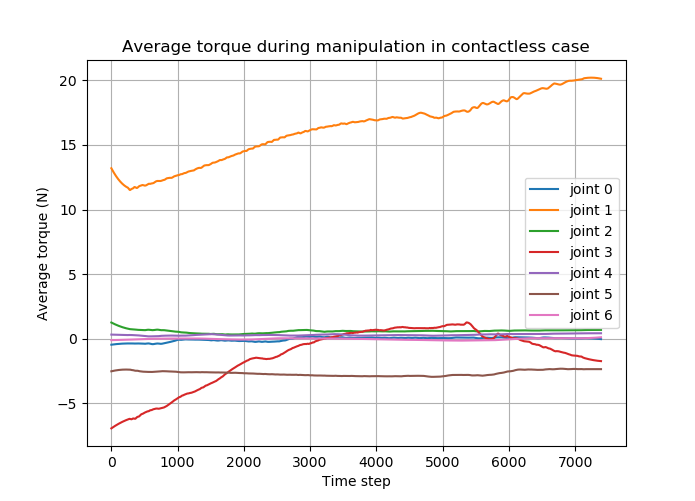
\includegraphics[width=1\textwidth]{images/us1_conless_tor.png}
          \caption{Average torque during manipulation in contactless case}
        \end{figure}
      \end{figure}
      \end{column}
      \end{columns}
  \end{frame}

  \begin{frame}{Experiement and evaluation}
    \framesubtitle{Perform writing task}
    \begin{columns}[c]
      \begin{column}{.5\textwidth}
        \begin{itemize}
          \item Compare the trajectory
          \item Accuracy is the maximum displacement
          in linear y direction
        \end{itemize}     
        \centering
        \begin{block}{Hypothesis}
          The accuracy will be increase, and the trajectory will be more stabile in contact case
        \end{block}

      \end{column}
      \begin{column}{.5\textwidth}
        \centering
        *insert demo video*
      \end{column}
      \end{columns}
  \end{frame}

  \begin{frame}{Experiement and evaluation}
    \framesubtitle{Perform writing task}
    \begin{columns}[c]
      \begin{column}{.5\textwidth}
        \begin{table}[H]
          \centering
          \resizebox{\textwidth}{!}{%
          \begin{tabular}{c|c|c|}
          \cline{2-3}
                                            & maximum displacements(m) & average displacements(m) \\ \hline
          \multicolumn{1}{|c|}{Contact}     &  0.00211145              & -0.00120878               \\ \hline
          \multicolumn{1}{|c|}{Contactless} &  0.00089509              &  0.00034292              \\ \hline
          \end{tabular}%
          }
          \caption{Table of the average displacement, and maximum displacement in contact and contactless case}
          \label{tab:us2_displacement}
          \end{table}
      
      \end{column}
      \begin{column}{.5\textwidth}
        \begin{figure}
          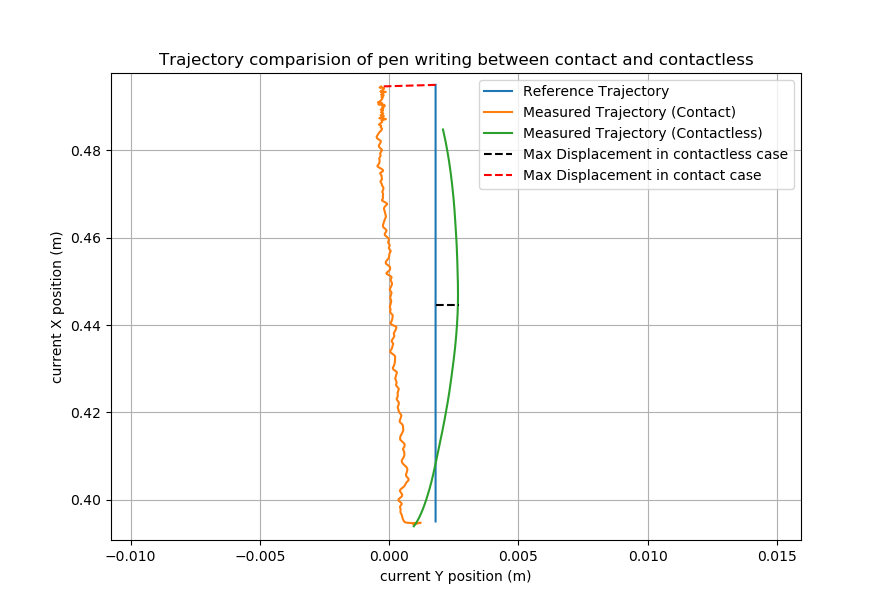
\includegraphics[width=1\textwidth]{images/us2_contactless_traj2.png}
          \caption{Average torque during manipulation in contactless case}
        \end{figure}
      \end{column}
      \end{columns}
  \end{frame}

  \begin{frame}{Experiement and evaluation}
    \framesubtitle{Resting elbow manipulation}
    \begin{itemize}
      \item A potential increase in energy efficiency by allowing \alert{certain joints of the manipulator} to rest on a supporting surface
    \end{itemize}
    \begin{block}{Hypothesis}
      The energy efficiency increases and 
      joint torque decrease in contact case
    \end{block}
  \end{frame}
  \begin{frame}{Experiement and evaluation}
    \framesubtitle{Resting elbow manipulation}
    \vspace{-3mm}
    \begin{columns}[c]
      \begin{column}{.5\textwidth}
        \begin{figure}
        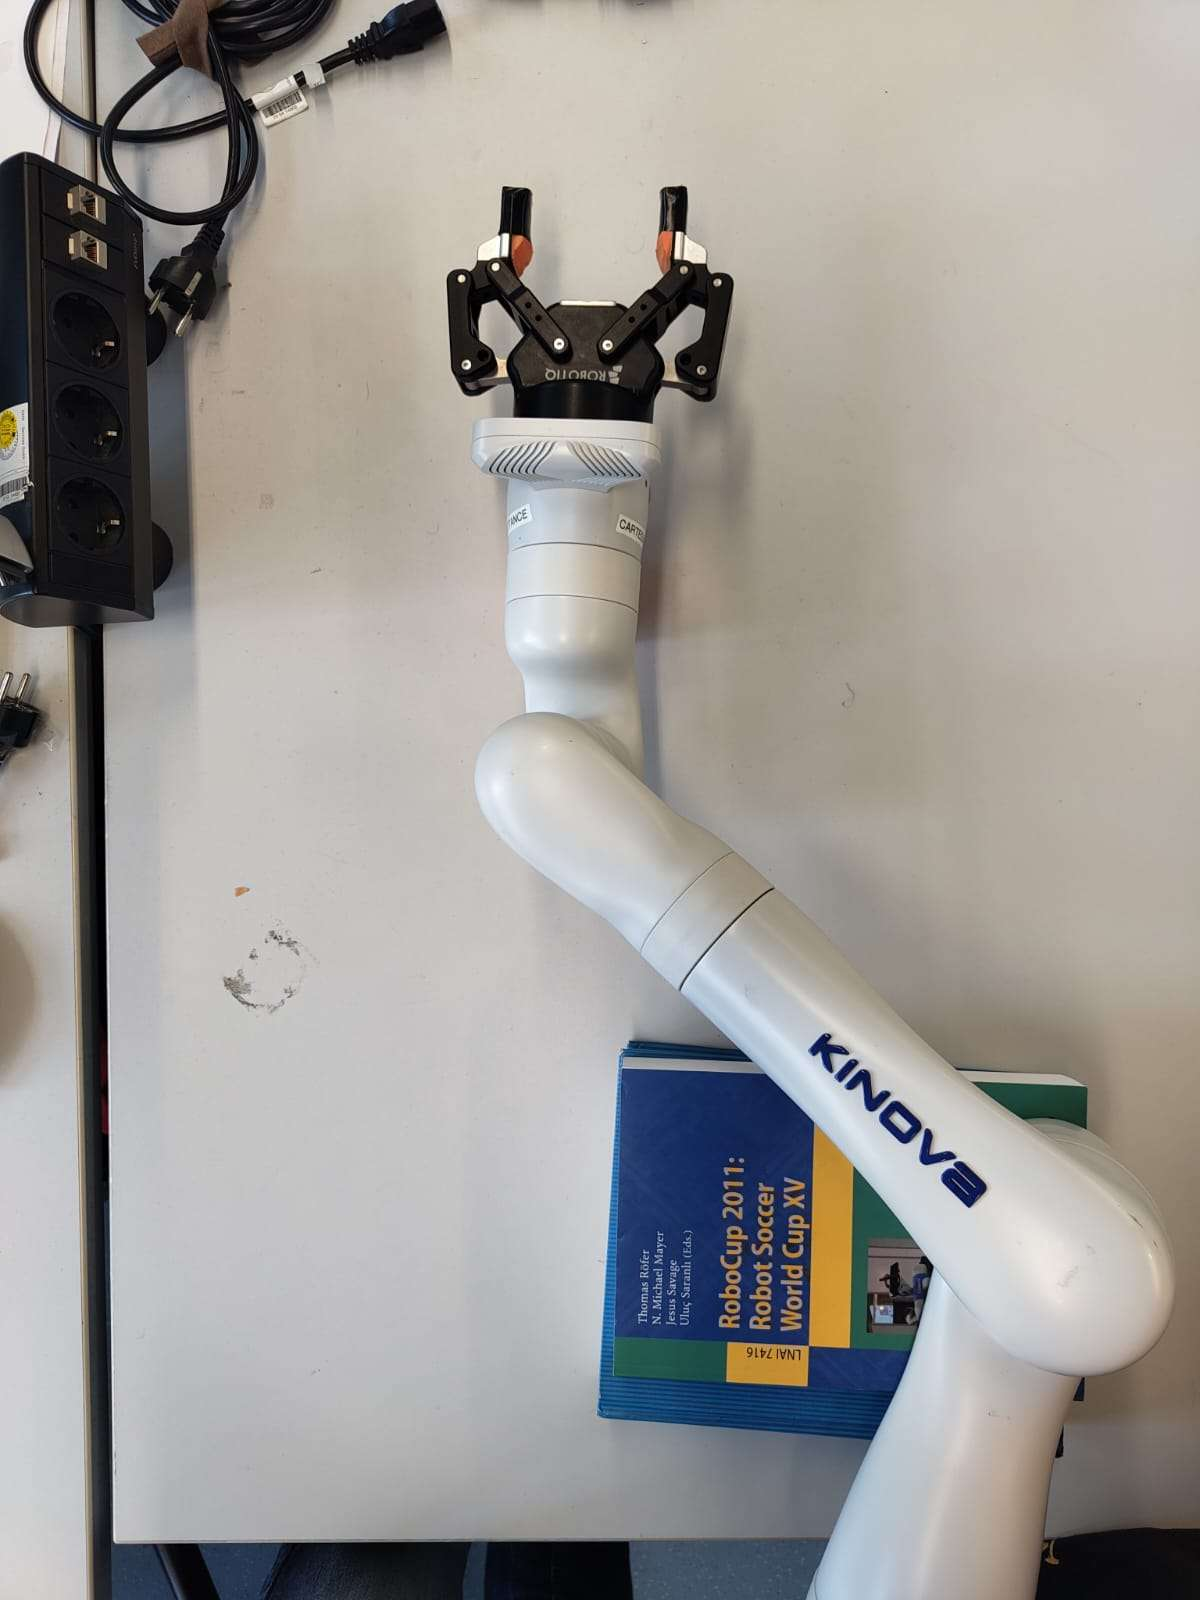
\includegraphics[width=0.6\textwidth]{images/us3_initial.jpg}
        \caption{The initial position of the robot arm in use case 3 where the elbow joint is resting on a book}
      \end{figure}
      \end{column}
      \begin{column}{.5\textwidth}
      \begin{figure}
        \centering
        \begin{figure}
          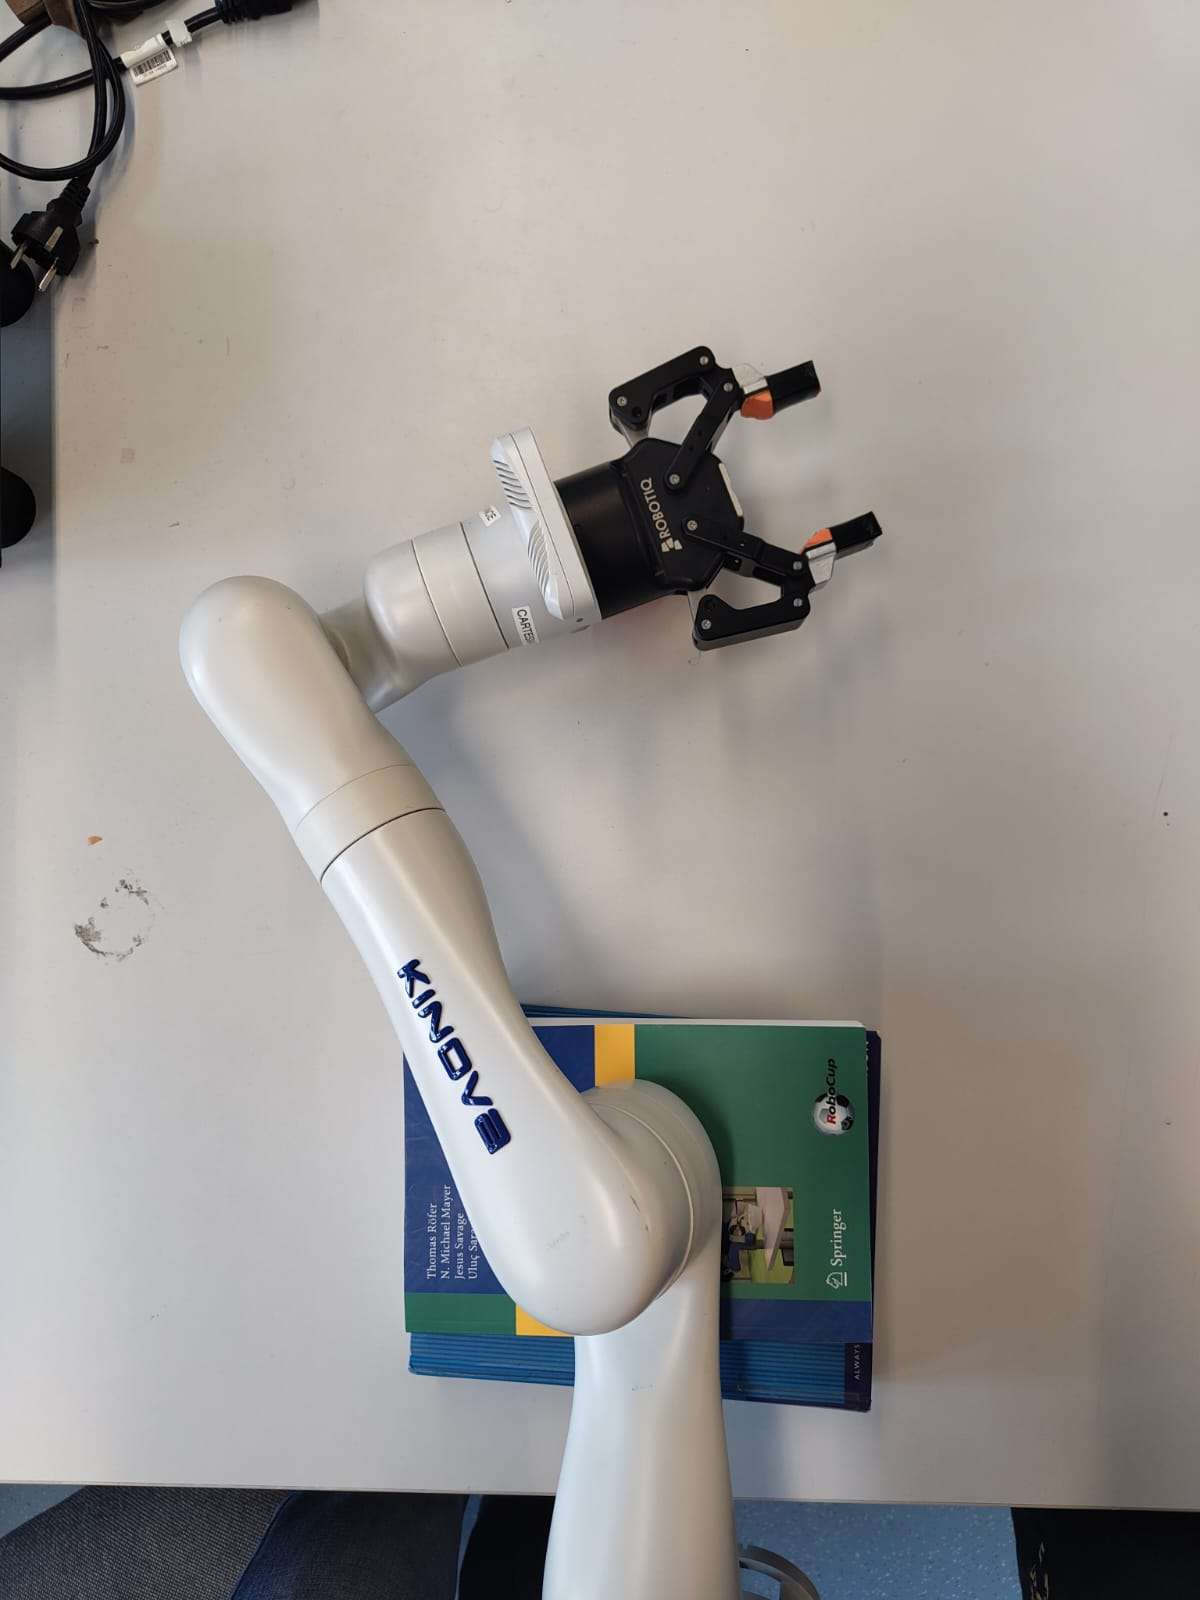
\includegraphics[width=0.6\textwidth]{images/us3_final.jpg}
          \caption{The final position of the robot arm in use case 3 where the elbow joint is resting on a book}
        \end{figure}
      \end{figure}
      \end{column}
      \end{columns}
  \end{frame}

  \begin{frame}{Conclusion}
    \begin{itemize}
      \item Background of related works on dynamic solver were introduced
      \item A cascaded controller is being implemented
      \item The Robif2b library is extened to retrieve voltage and current status of each joint
      \item Three experiements were conducted
      \item Average energy consumption and joint torque of most of the robot’s joints \alert{decreased}
      \item The accuracy of motion in contact scenarios was found to be \alert{lower}
    \end{itemize}
  \end{frame}


  \begin{frame}{Future work}
    \begin{itemize}
      \item Study on how \alert{different tasks and contact surface} affect the
      energy consumption of the robot manipulator
      \item Fuse force/torque sensor on the robot manipulator
    \end{itemize}
  \end{frame}
% \subsection{Structuring Elements}
%     \begin{frame}[label=simmonshall]{Text blocks}
%       \framesubtitle{In plain, example, and \alert{alert} flavour}
%       \alert{This text} is highlighted.

%       \begin{block}{A plain block}
%         This is a plain block containing some \alert{highlighted text}.
%       \end{block}
%       \begin{exampleblock}{An example block}
%         This is an example block containing some \alert{highlighted text}.
%       \end{exampleblock}
%       \begin{alertblock}{An alert block}
%         This is an alert block containing some \alert{highlighted text}.
%       \end{alertblock}
%     \end{frame}


    \begin{frame}[allowframebreaks]{Bibliography}
      % \nocite{*}
      \printbibliography
    \end{frame}


% \section{Something else}

% \begin{frame}
% \frametitle{There Is No Largest Prime Number}
% \framesubtitle{The proof uses \textit{reductio ad absurdum}.}
% \begin{theorem}
% There is no largest prime number. \end{theorem}
% \begin{enumerate}
% \item<1-| alert@1> Suppose $p$ were the largest prime number.
% \item<2-> Let $q$ be the product of the first $p$ numbers.
% \item<3-> Then $q+1$ is not divisible by any of them.
% \item<1-> But $q + 1$ is greater than $1$, thus divisible by some prime
% number not in the first $p$ numbers.
% \end{enumerate}
% \end{frame}

% \begin{frame}{A longer title}
% \begin{itemize}
% \item one
% \item two

% \textbf{This is a test of bold text}

% \end{itemize}
% \end{frame}

% \begin{frame}[allowframebreaks]{Test}
%   First slide
%   \begin{itemize}
%     \item
%     \item
%     \item
%     \item
%     \item
%   \end{itemize}
%   \framebreak
%   Second slide
%   \begin{itemize}
%     \item
%     \item
%     \item
%     \item
%     \item
%   \end{itemize}
% \end{frame}
%--- Next Frame ---%



\end{document}
